\chapter{Introduction}
\section{Motivation}
Since the introduction of Bitcoin, a peer-to-peer payment network and cryptocurrency, there have been countless new cryptocurrencies that are used and traded. Along with this, their high volatility has piqued a lot of retail investor's interest with some investors gaining a high return of interest and others losing a lot of money~\cite{losing_money_on_crypto_2021}. In addition to this, larger investment institutions have also sought to gain profits from this new type of tradable asset~\cite{gondek_what_nodate}. This has lead to more sophisticated forms of cryptocurrency trading.
\\[5mm]
However, trading cryptocurrencies was initially very difficult for people without technical know-how, and the first recorded transaction was on $12^{th}$ October 2009 via a paypal transaction~\cite{noauthor_history_nodate}. Since then, other cryptocurrency exchanges have emerged, many of which are centralized, which provide a more traditional trading terminal and support for investors with little technical know-how, and others are decentralised, which operate on blockchain networks and allow users to directly with each other using smart contracts. Centralized exchanges are predominant due to their easy-to use and familiar interface for traders. We can see in Figure \ref{fig:dex_to_cex} the proportion of trades on decentralised exchanges compares to the number of trades on centralized exchanges, we can also see that the volume traded in DEXes have been near 0\% until the summer of 2020 and has been increasing since. 

\begin{figure}[htb!]
    \centering
    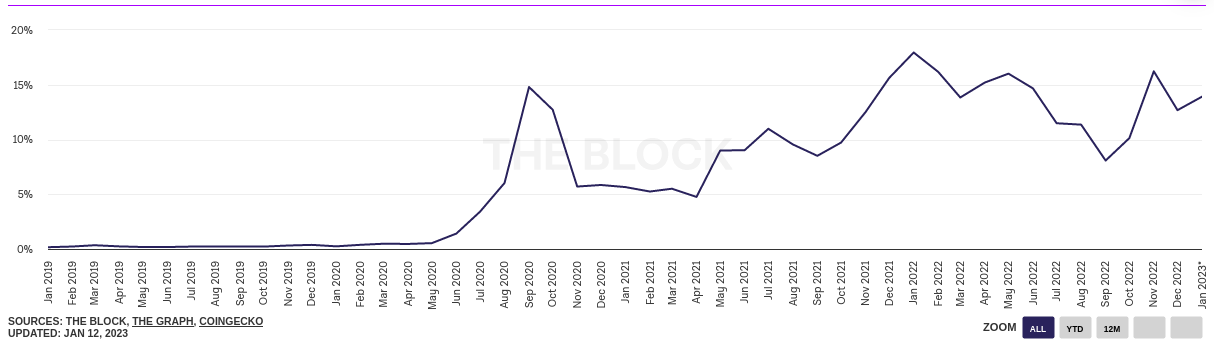
\includegraphics[width=\textwidth]{introduction/Images/dex_to_cex.png}
    \caption{{DEX} to {CEX} {Spot} {Trade} {Volume}~\cite{dex_to_cex}}
    \label{fig:dex_to_cex}
\end{figure}

This poses the question that about which trading strategies can exploit arbitrage opportunities on decentralised exchanges. There has been some research on this topic, mainly focussing on triangular and cyclic arbitrage on DEXes such as Uniswap and SushiSwap, however there has been no research into analysing the performance of statistical arbitrage methods on decentralised exchanges.

% \section{Objectives}
% The objectives for this project is to design, implement and analyse the performance of numerous statistical arbitrage strategies.
% \subsection{Example of Statistical Arbitrage}
% Before outining the objectives, it is important to understand the process of statistical arbitrage. The process in which statistical arbitrage is executes is in 3 steps:
% \begin{enumerate}
%     \item Identify a pair of assets that are cointegrated/correlated, i.e. follow the same trend and have a similar mean
%     \item When the prices diverge, long the undervalued asset and short the overvalued asset.
%     \item When the prices then revert back to it's mean, close the position.
% \end{enumerate}
% An example of the price dynamic of one such pair can be seen in Figure \ref{fig:stat_arb_example}.

% \begin{figure}[htb!]
%     \centering
%     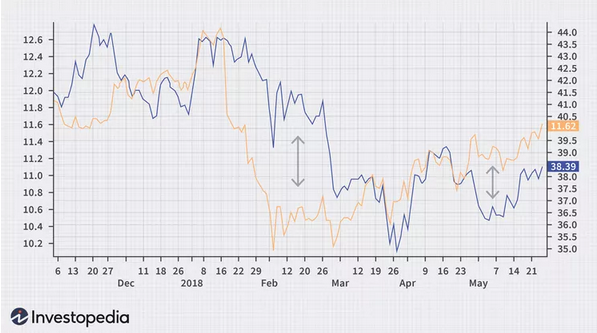
\includegraphics[width=0.8\textwidth]{introduction/Images/stat_arb_example.png}
%     \caption{Stock Prices of General Motors and Ford Motor Company~\cite{noauthor_statistical_nodate}}
%     \label{fig:stat_arb_example}
% \end{figure}

% \subsection{Objectives and Contributions}
% As previously mentioned, I will be implement and analyse numerous trading strategies:
% \begin{itemize}
%     \item \textbf{Simple Mean Reversion Strategy}
%     \item \textbf{Mean Reversion Strategy using the Kalman Filter to calculate the hedge ratio}
%     \item \textbf{Machine Learning Forecasting with the Kalman Filter}
% \end{itemize}

\section{Contributions - TODO}